\documentclass[10pt,letterpaper]{article}

%\usepackage{cogsci}
\usepackage{pslatex}
\usepackage{apacite}
\usepackage{color}
\usepackage{amsmath}
\usepackage{amsfonts}
\usepackage{amssymb}
%\usepackage{widetext}
\usepackage{graphicx, caption, subcaption}
% subfig
\usepackage{fixltx2e}


%%%% biblatex-apa
%\usepackage[american]{babel}
%\usepackage{csquotes}
%\usepackage[style=apa,hyperref,doi,url]{biblatex}
%\DeclareLanguageMapping{american}{american-apa}
%\bibliography{tec_references}


\numberwithin{equation}{section}

\title{A continuous time neural model for sequential action}

\author{George Kachergis$^1$, Dean Wyatte$^2$, Randall C. O'Reilly$^2$, \\
	Roy de Kleijn$^1$, and Bernhard Hommel$^1$ \\
	\bf george.kachergis@gmail.com \\
	$^1$ Institute for Psychological Research \& \\
	Leiden Institute for Brain and Cognition, Leiden University \\
	$^2$ Department of Psychology and Neuroscience, \\
	University of Colorado Boulder }

\date{}

\begin{document}
\maketitle


%%%%%%%%%%%%%%%%%%%%%%%%%%%%%%%%%%%%%%%%%

\sloppy

\section*{Abstract}

Action selection, planning, and execution are continuous processes that evolve over time, responding to perceptual feedback as well as evolving top-down constraints. Existing models of routine sequential action (e.g., coffee- or pancake-making) generally fall into one of two classes: hierarchical models that include hand-built task representations, or heterarchical models that must learn to represent hierarchy via temporal context, but lack goal-orientedness. We present a biologically-motivated model of the latter class that, because it is situated in the Leabra neural architecture, affords an opportunity to include both unsupervised and goal-directed learning mechanisms.  Moreover, we embed this neurocomputational model in the theoretical framework of the Theory of Event Coding (TEC), which posits that actions and perceptions share a common representation with bidirectional associations between the two. Thus, in this view, not only does perception select actions (along with task context), but actions are also used to generate perceptions (i.e., intended effects). We propose a neural model that implements TEC to carry out sequential action control in hierarchically structured tasks such as coffee-making. Unlike traditional feedforward discrete-time neural network models, which use static percepts to generate static outputs, our biological model accepts continuous-time inputs and likewise generates non-stationary outputs, making short-timescale dynamic predictions. 

\section*{Introduction}

Action control is essential to the daily routines of life, being an integral part of everyday activities from getting dressed to making pancakes. Yet, in our effort to distill cognitive processes in the laboratory, our controlled experiments often remove many of the interesting aspects of voluntary action. Although arbitrary stimulus-response experiments have in fact granted much insight into basic cognitive mechanisms of perception, learning, and decision-making, as engineers endeavor to build humanoid robots to accomplish everyday cooking and cleaning tasks \cite<e.g.,>{Tenorth:2013}, the field of cognitive psychology seemingly has embarrassingly little advice to offer. Despite early interest in how an action precipitates from thinking of its to-be-achieved effects, or goal \cite<e.g.,>{James:1890}, the more mainstream sensorimotor paradigm investigates the reverse: stimuli-driven perception resulting in action. From the sensorimotor perspective \cite<e.g.,>{Donders:1868,Sternberg:1969}, the stimulus is seen as the driving force behind the subsequent selection, preparation, planning, and execution of an action. However, the sensorimotor approach is difficult to extend to the broader arena of goal-directed action, where desired effects can lead executive function to initiate appropriate actions. 

The Theory of Event Coding \cite<TEC;>{Hommel:2001} takes this ideomotor perspective and additional principles to explain a wide variety of action control phenomena \cite{Hommel:2009}. TEC emphasizes that task context is important for selecting which features are emphasized, and which are ignored. Indeed, perceived features such as size and location can directly influence actions--beyond cognitive control, as seen in stimulus-response compatibility phenomena such as the Simon effect \cite{Simon:1967}. This implies there is a direct route from perception to action, bypassing cognition and many of the sensorimotor view's steps of planning, selection, and preparation. TEC's premise that perception and action plans share a common representation allows percepts--along with task context--to directly generate and select actions. Since action effects also share this common coding, desired effects (i.e., goals) can activate relevant actions to achieve the effect \cite{Elsner:2001}. It turns out that TEC is underspecified, however, for it was originally conceived as a meta-theoretical framework mainly concerned with simple one-step, ballistic actions. This lack of specificity becomes more obvious when considering the complexities of everyday action, which are thought to require sequential, hierarchically-structured goals. 

%In this paper we offer a general, biologically-motivated model of sequential action learning stemming from the Leabra cognitive architecture. Further, we situate this model in TEC, a theoretical framework which distinguishes it from existing models, promising to offer the best of the previous schema-based and recurrent approaches. 

In this paper, we present a computational model of sequential action learning, stemming from the biologically-motivated Leabra cognitive architecture \cite{OReilly:2000,OReilly:book}. We show how this model implements the central principles of TEC, and situates it in a biological and ecological context. We address two key questions: 1) How might goals be represented? and 2) Do multi-step, nested actions require hierarchical representations? Both questions are important because TEC assumes that goals have strong impact but it is not specific as to how the goal is represented. It also seems to suggest that goal representation is implicit \cite<i.e., the goal is represented by the way it affects the system: e.g., weighting features according to their importance for achieving the goal>{Memelink:2013}. Leabra fills out this missing information and gives a concrete explanation of how goals can be implicit and yet yield feedback for learning.

We begin by reviewing TEC and previous attempts at modeling everyday action, focusing on ways to integrate theoretical, empirical, and biological constraints. We then propose how Leabra can resolve some of the remaining constraints by representing proximal goals as implicit task context in separate neural subpopulations. Because goals and actions share a common coding, error-driven learning can be used to learn associations between subsequent actions. We describe a proof-of-concept neural model that demonstrates how these mechanisms can account for everyday action in a coffee-making task. 

\section*{Theory of Event Coding}

TEC is a theoretical framework that describes how an agent's actions and perceptions are remembered, and how these memories are used to generate future actions (and thus perceptions). TEC assumes that perception and actions are represented using the same feature codes, which encode relevant aspects of the environment (e.g., color, size, location, shape), and not merely proximal features. Thus, activation of feature codes that represent distal events is an integral part of both perception and action planning. The assumption that feature codes are used to represent both the properties of a response as well as those of a stimulus in the environment is derived from ideomotor theory, which states that actions are represented in terms of their perceivable effects \cite{James:1890,Stock:2004}. When an action is executed, the motor pattern becomes associated with the perception of the action's effects. \citeA{Elsner:2001} explored this in a series of experiments, finding that keypresses (i.e., actions) producing particular auditory tones were later primed by hearing the corresponding tone, demonstrating that the learned action-effect association also works when temporally reversed.

The universal representation proposed by TEC, called an event code (or event file), represents features of the environment rather than proximal features of the sensation (e.g., auditory intensity). For example, consider a version of the \citeA{Simon:1967} task, in which subjects are asked to respond with a left or right keypress to target color patches (e.g., green or red), which appear either on the left or right of the screen. Although the spatial location is irrelevant to the response, subjects respond faster and more accurately when the target requires a compatible response (left stimulus and left response, or right stimulus and response), in comparison to incompatible responses (left stimulus and right response or vice-versa). TEC accounts for this effect because when a perception (green, left side) activates a feature (e.g., left) that is shared with an action, that action (e.g., left keypress) is primed. That is, the event code is the integrated assembly of distal sensorimotor features (e.g., spatial location, color) that are relevant for perception and action, integrated with task context. The development of an event file enables low-level action planning, for once an action becomes associated with a distal effect, the desire to achieve an effect activates the action. Further evidence for shared representational resources comes from studies showing that verifying perceptual properties from the same modality (e.g., sight: color and luminance) results in processing advantages, compared to properties from different modalities--whether it is for the same object, or different objects \cite{Pecher:2003,Pecher:2004}. This supports the idea that sensorimotor simulations are involved in representing concepts, a central tenet of TEC and of perceptual symbol systems, in general \cite{Barsalou:1999}.

% There is mounting evidence that the motivation for approach and avoidance behaviors is not simply a matter of a stimulus' presence; rather, it is a function of the expected outcomes of the behavior, given the stimulus \cite<i.e., the goal; >{Eder:2013}. This might seem patently obvious given a simple example: seeing a donut will not stimulate an approach behavior in a person who has just eaten several donuts, and is now thirsty rather than hungry. Thus, according to \citeA{Eder:2013}, behaviors should be controlled by anticipation of desired (or undesired) outcomes. Actions that produce desired outcomes should become associated to the stimulus--but only in the context of the agent's current desires. % Bernhard removed 12/1

The core principles of TEC have been instantiated in HiTEC \cite{Haazebroek:2011}, a connectionist model composed of sensory-motor, feature, and task levels. While this initial model proved that the basic tenets of TEC are sufficient to account for a wide variety of experimental compatibility effects--as has been predicted by TEC--HiTEC does not yet provide a fully general account of how feature and task codes can be learned from experience. Moreover, although TEC explains simple goal-directed action in addition to the standard sensorimotor stimulus-response account, it has not yet been extended to sequences of actions, which are typical in everyday tasks, let alone hierarchies of tasks and goals.


\section*{Modeling everyday action}

Learning everyday actions is generally agreed to be complex, for actions are experienced serially, and yet are typically thought of as hierarchical since some subactions (e.g., mixing in eggs) are part of multiple actions (e.g., making pancakes or cookies). Moreover, these shared subactions may precede or follow distinct actions. \citeA{Lashley:1951} pointed out that the bulk of human sequential actions cannot be explained by merely associating perceptual inputs and actions, since the prior action and the current percepts do not sufficiently constrain action selection \cite<for a review, see>{Rosenbaum:2007}. Rather, a more elaborate representation of task context is needed, that persists through multiple actions and helps select the appropriate next action. For example, when a baker sees a bowl of cake batter, he may need to know whether he is making cupcakes or a cake--the high-level goal--in order to perform the next action: pouring the batter in an appropriate receptacle. Task structure is typically defined by researchers as hierarchical, since everyday tasks such as tea- and coffee-making often contain subtasks such as adding cream or adding sugar that are discrete and interchangeable.

Thus, action selection for everyday tasks requires representing the task context in a way that preserves both the high-level task, as well as appropriate subtasks. In schema-based models, this multilevel task context is built-in via hand-coded hierarchical representation of the task structure \cite<e.g.,>{Cooper:2000,Cooper:2006}. The strength of schema-based models could be argued to be their explicit representation of goals and subgoals as nodes in a task hierarchy that is comprehensible to researchers, if perhaps not laymen. Many robotic systems use schema-based architectures: despite the need to hand-code much of the representation, roboticists may find it worth the certainty of knowing how exactly the system will react to any given set of conditions, rather than reacting stochastically and perhaps unpredictably. Given researchers' strong belief in the hierarchical structure of everyday tasks, and that the cognitive representation likely mirrors this compositional structure, we must ask how the structure of complex everyday actions can be learned by the human system: is it necessary to explicitly build hierarchy into the representation?

Ultimately, a realistic model needs be able to learn the general task structure from a series of exemplars, much like the learning problem humans face. A model that extracts the semi-hierarchy of a task should allow more natural generalization to new tasks, since subsequences at the appropriate level will be seen to be quite similar, and thus shared.  How can a model represent task context during temporally-extended task execution, in a way that also supports learning of these structures via experience? \citeA{Botvinick:2004} introduced a connectionist model that encodes context at multiple timescales. Essentially, the model is a simple recurrent network \cite<SRN;>{Elman:1990} consisting of three groups of neurons arranged in a loop: perception, internal, and action. The perception group receives input from the simulated environment (e.g., ``sugar packet''), and the action group outputs simple actions (e.g., ``pick up cup'') that modify the environment (and thus, the next percept). The hidden internal neuron group is recurrent, allowing it to come to represent temporal context, possibly representing previous states of the environment. The SRN model performs well at an instant coffee making task, which consists of four subtasks: adding coffee, adding cream, adding sugar (from a bowl or paper packet), and drinking. Each of these subtasks is comprised of several simple actions, such as picking up, putting down, and pouring. This model was shown to be able to generalize to tea-making--which shares subactions such as adding sugar--without catastrophic forgetting. The SRN model is trained via back-propagation through time \cite{Williams:1995}, and shows many of the same substitution and omission errors that humans commit.

%In contrast to the SRN model \citeA{Botvinick:2004} which has no explicit hierarchy nor goals in its representations, \citeA{Cooper:2006} argued that  hierarchical organization with goals represented in schemata are necessary to explain sequential behavior. The proposed interactive activation network (IAN), following \citeA{Cooper:2000}, is a hybrid of connectionist networks representing ... with symbolic rules.

\citeA{Botvinick:2004} demonstrates that it is possible to learn hierarchically-structured actions from training on sequential actions, and without hierarchy built into the model. Further, \citeA{Botvinick:2007} argues that strictly hierarchical models cannot account for context-sensitivity. For example, you might add different types and amounts of sugar to different beverages (coffee or tea). Do you then need different schema nodes for every type of sugar-adding? If you have multiple nodes, then how do you also encode the similarities between sugar-adding for these different beverages? Recurrent connectionist models, with spreading activation over distributed representations, allow similar sequences to develop similar representations, producing generalization as a natural byproduct. However, although the SRN model provides a first proof-of-concept for representing hierarchical everyday action without hierarchy, it lacks both biological foundations and any account of goal-directed behavior. 

TEC got away without a complex representational structure because in single-step actions, a goal is equivalent to the outcome of the action, which is often not the case when several steps are necessary to reach the goal. However, Leabra shows that it is fortunately unnecessary to give representations complex structure in TEC: hierarchically structured actions can be produced without hierarchy in the representations, much like the SRN. % The Leabra model we present in the next section explains how goals can be implicitly represented to some extent, and how hierarchical actions can be produced by nonhierarchical representations. Thus, it is not neccessary to give representations complex structure in TEC: hierarchically structured actions can be produced without hierarchy in the representations, much like the SRN. The Leabra model we present in the next section explains how goals can be implicitly represented to some extent, and how hierarchical actions can be produced by nonhierarchical representations.


\section*{Learning sequential actions with Leabra}

Leabra (Local, Error-driven and Associative, Biologically Realistic Algorithm) is a general model of the neocortex that incorporates many widely-accepted biological principles of neural processing and has been used to successfully implement a growing number (50+) of models and tasks \cite{OReilly:2000,OReilly:book}. Leabra models the brain at scales ranging from individual neurons up to the structural organization of macroscopic areas, and makes predictions regarding the neural mechanisms, time course, and substrates of cognitive processing. Models consist of a homogenous set of mechanisms including a biological integrate-and-fire neuron model \cite{Brette:2005}, \textit{k}-winners-take-all inhibitory competition, and deep architectures with bidirectional excitatory synapses. Most parameter settings are consistent across models and thus, the model described here can be viewed as a specific instantiation of a systematic modeling framework opposed to a model with completely new mechanisms.


Learning in Leabra models is traditionally accomplished by a biphasic algorithm that incorporates self-organizing Hebbian and error-driven components derived from synaptic LTP/LTD mechanisms. For the error-driven component, the network state is said to be in the \emph{minus phase} when representing a prediction, and the \emph{plus phase} when an actual outcome occurs. In learning to represent temporally ordered properties such as action sequences, a model must be able to generate the state at time \textit{t} using the representation from time \textit{t-1}. Leabra's error-driven learning makes this difficult, since synaptic weights are updated to minimize the difference in neural activations across the minus and plus phases, which are assumed to occur in sequence. To address this difficulty, we have extended the Leabra learning algorithm to make predictions about time \textit{t} by explicitly representing information from time \textit{t-1} and integrating errors over these two periods. We refer to this extension as LeabraTI (Temporal Integration; O'Reilly, et al., in preparation).

% Cortex is arranged in six layers of neurons that are interconnected in a fairly characteristic pattern (see Figure 1a). Different areas of cortex have specialized function and can thus emphasize different layers \cite{OReilly:book}. Areas of cortex that receive sensory input (e.g., primary visual cortex) receive it via the thalamococortical projections to enlarged layer 4. In contrast, primary motor cortex emphasizes deep layers 5/6, which are hidden from receiving direct sensory input and project into subcortical areas (e.g., the basal ganglia) to drive motor responses. Prefrontal cortex, associated with executive function, has equal thickness in all layers.  

LeabraTI is closely related to the traditional SRN architecture, which explicitly represents the previous time step's information in a population of ``context'' neurons. Accomplishing this property in biological neural circuits that are continuously updated requires a mechanism to gate information into a relatively isolated sub-population of neurons. In LeabraTI, a thalamocortical circuit extending vertically through the layers of a local microcolumn of 80-100 neurons \cite{Mountcastle:1997,Douglas:2004} accomplishes this operation (Figure \ref{fig:leabrati}a). Specifically, sensory input enters cortex through the thalamus in Layer 4 and is transmitted to superficial layers (Layers 2 and 3). From there information is both propagated downstream to Layer 4 of the secondary cortical area, as well as to deep layers of the local microcolumn (Layers 5 and 6), which we believe serve as a temporal context representation as they are relatively isolated from extra-columnar inputs. 

\begin{figure}[h]
\centering
\begin{tabular}{ll}
a) & b) \\                
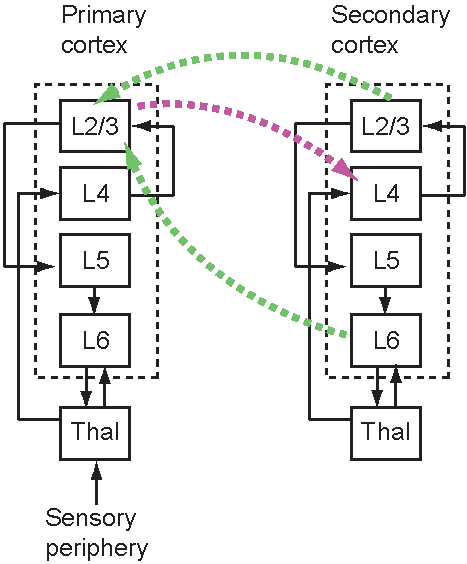
\includegraphics[width=0.49\textwidth]{figs/microcircuit_horiz} & 
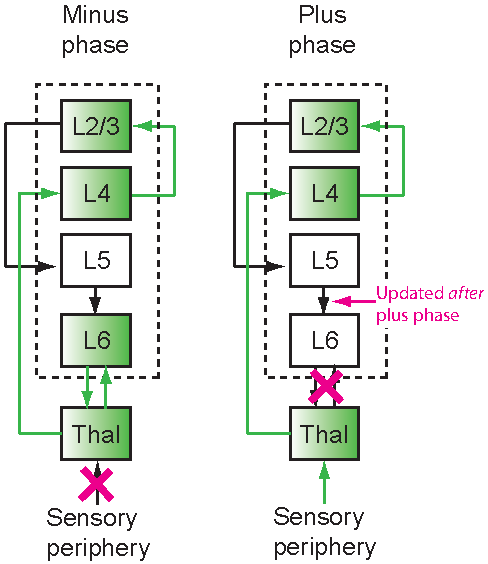
\includegraphics[width=0.51\textwidth]{figs/microcircuit_minus_plus} \\
\end{tabular}
\caption{\small{Neocortical anatomy supporting LeabraTI. a) Cortical areas are composed of microcolumns with canonical circuitry within and between areas. Within a microcolumn, information follows the path Layer 4 $\rightarrow$ Layer 2/3 $\rightarrow$ Layer 5 $\rightarrow$ Layer 6. Layer 2/3 sends feedforward projections to the next area and are the primary site of feedback, and thus can be seen as doing bidirectional information processing. b) Layer 5 neurons integrate contextual information from Layer 2/3 $\rightarrow$ Layer 5 synapses, and gate this context signal into Layer 6 neurons. These Layer 6 neurons sustain the context via recurrent projections through the thalamus, which also recirculate the context through the local microcolumn to support generation of the next prediction during the minus phase. Veridical information from the sensory periphery drives the microcolumn in the plus phase. Layer 6 context is not used during the plus phase, but is updated through the Layer 2/3 $\rightarrow$ Layer 5 $\rightarrow$ Layer 6 intra-columnar circuit at the end of processing (roughly every 100 ms).}}
\label{fig:leabrati}
\end{figure}

To generate useful predictions, temporal context must be integrated and stored over a short timescale. LeabraTI predicts that this occurs over roughly 100 ms intervals, in line with the intrinsic bursting properties of Layer 5 neurons \cite{Connors:1982,Silva:1991}.  Specifically, predictions in the minus phase, driven by temporal context from Layer 6 to Layer 4 transthalamic synapses, are interleaved with actual information from the sensory periphery transmitted through the thalamus to Layer 4 during the plus phase. Temporal context in deep layers is updated at the end of the plus phase with the current sensory information. The difference between the minus and plus phases is used to update both the interareal synaptic weights as well as the intracolumnar Layer 5 to Layer 6 synaptic weights, allowing the network to jointly learn the current input as well as the mapping between subsequent inputs. The overall LeabraTI computation is depicted in Figure \ref{fig:leabrati}b. For computational efficiency, we do not explicitly model Layer 4 $\rightarrow$ Layer 2/3 or Layer 2/3 $\rightarrow$ Layer 5 intra-columnar synapses and instead assume that they are perfect one-to-one relays. This reduces the complexity of the model to bidirectionally connected superficial (Layer 2/3) layers with corresponding deep (Layer 6) layers that sustain the previous moment's context over 100 ms periods. 


\subsection*{Model of coffee-making task}
% A Leabra model was built using the Emergent modeling system \cite{Aisa:2008} to test LeabraTI on a coffee-making task. 


We built a model incorporating the general LeabraTI architecture to perform a coffee-making task that has been targeted by other recent models of sequential action \cite<e.g.,>{Cooper:2000,Botvinick:2004}. Making instant coffee or tea is a suitable everyday task to study sequential action, for it is composed of a number of subtasks (e.g., adding sugar) that may be performed in varying order and number of repetitions. For training, we used a formalization similar to that used by \citeA{Botvinick:2004}, using features to describe the currently fixated object, held object, and performed actions (e.g., a step: fixate 1-handled cup with clear liquid, holding nothing, and now fixate the coffee packet). However, instead of using a few fixed training orders like \citeA{Botvinick:2004}, we wrote a finite state grammar to generate reasonable sequences of actions (see below). 

The model architecture is depicted in Figure \ref{fig:coffeenet}. The model contains three sensorimotor layers (Visual, Manual, Action; 25 neurons each) bidirectionally connected to a hidden layer, which is in turn connected bidirectionally to a second hidden layer (64 neurons each). Context layers are composed of the same number of neurons as their superficial counterparts, doubling the number of units in the network. All connections in the model, including those between superficial and deep layers , are are all-to-all, connecting each unit in the receiving layer to every unit in the sending layer. Context is stored by filtering the state of superficial layers at the end of the plus phase through the superficial-to-deep weights and applying it as an additional graded input to the receiving area during the minus phase.
%This second hidden layer is isolated from the sensorimotor layers, and thus can serve as a stable memory, and perhaps come to represent higher-level task context. 

\begin{figure}[h]
  \centering
  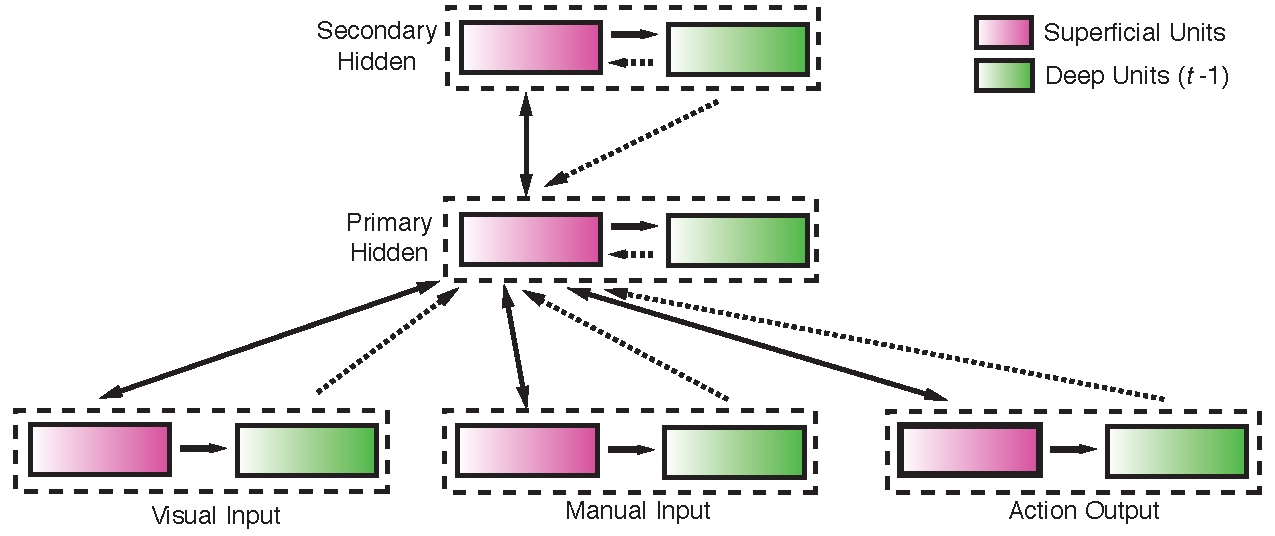
\includegraphics[width=\textwidth]{figs/coffee_tea_arch}
  \caption{\small{Network architecture for the coffee tea simulation. Similar to \protect\citeA{Botvinick:2004}'s SRN model of this task, the input is divided into visual and manual perceptual layers, feeding into a recurrent hidden layer, which in turn drives another hidden layer that is not connected to the sensorimotor layers. Note that each layer in a LeabraTI network has both a superficial layer (purple) and a corresponding deep layer (green). Superficial layers can only project to superficial layers (and their own deep layer), but deep layers can project to any superficial layer. Deep layers receive only projections from their own superficial layer.}}
  \label{fig:coffeenet}
\end{figure}

The Visual layer represents 19 features: the cup, 1-handle, 2-handle, lid, clear liquid, brown liquid, light, carton, open, closed, foil, paper, torn, untorn, spoon, teabag, sugar, and empty. The Manual layer represents all 19 of the features in the Visual layer, with the addition of 'nothing' (i.e., an empty hand). The Action layer represents 19 actions: pick up, put down, pour, peel open, tear open, pull open, pull off, scoop, sip, stir, dip, say ``Done'', fixate cup, fixate coffee packet, fixate spoon, fixate carton, fixate sugar packet, and fixate sugar bowl. These basic sensorimotor features can combine into 67 task-relevant steps which can be grouped into subactions. A finite state grammar was created to generate plausible coffee- or tea-making subaction sequences for training. Coffee-making sequences consist of adding coffee grounds, and then adding cream and sugar (if desired) in either order. Sugar can come from a packet or from a bowl, and may be added multiple times. Finally, the beverage is drunk. For the tea-making task, the teabag is steeped, an amount of sugar may be added from a packet or bowl, and the tea is drunk.

The model was trained using the LeabraTI extension of the Leabra algorithm %(see Appendix for details) 
for 200 epochs of 50 time steps. These time steps were generated from the finite state grammar of coffee- and tea-making subactions defined above, and the model iterated over these steps and adjusted connection weights according to LeabraTI. We trained 10 networks with randomly-initialized weights for 200 epochs (i.e., 10,000 trials per network). The mean SSE and number of errors per epoch during training for 10 simulated networks is shown in Figure \ref{fig:epochs}.  After training, accuracy on the coffee-making task was 96\% (SSE = .05). 

\begin{figure}
  \centering
  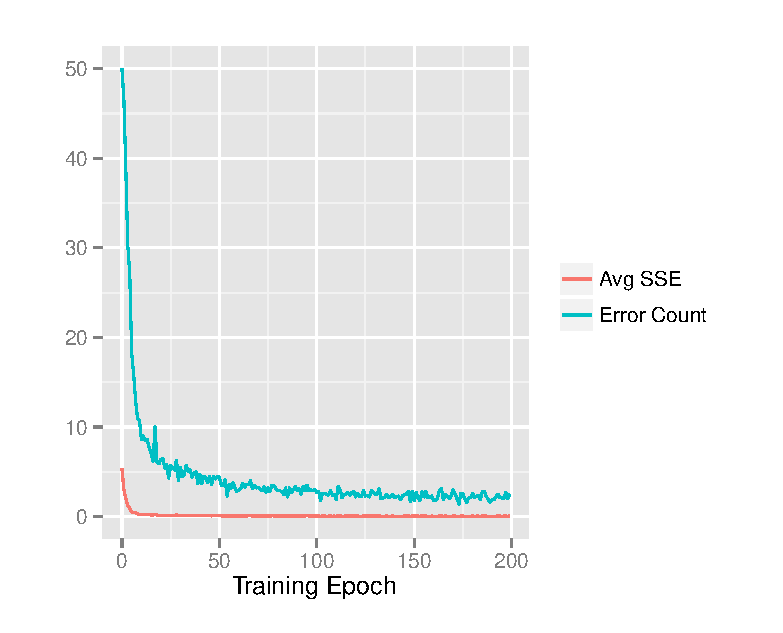
\includegraphics[width=0.8\textwidth]{figs/SSE_and_errors_vs_epoch}
  \caption{Mean SSE and number of errors per epoch during training for 10 simulated networks.}
  \label{fig:epochs}
\end{figure}

The model differs from previous SRN models in several ways. First, each layer input modality contains its own implicit context representation opposed to a single shared context representation attached to the hidden layer. This allows the model to learn more quickly and more robustly by learning visual-specific or manual-specific errors before integrating them into the hidden layer and its corresponding context. The model also has a second hidden layer \cite<though see>{Botvinick:2007}, which provides minimal structural hierarchy, granting our model greater power in representing nuanced context differences by learning what information to preserve or update over time. The bidirectionality of projections between the hidden layer and the sensorimotor layers sets our model apart from the sensorimotor-loop style of the SRN, bringing it in accord with TEC's ideomotor principle.

The LeabraTI model also makes use of a biologically tractable learning rule compared to the SRN model of \citeA{Botvinick:2004}, which was trained using backpropagation through time \cite<BPTT;>{Williams:1995}. BPPT requires the entire network to be unfolded through all of the steps in the action sequence before averaging the weights together which is computationally inefficient and relatively implausible as far as the brain is concerned. LeabraTI is capable of learning in a step-wise fashion in real time, synchronized with sensory inputs and action outputs. LeabraTI also appears to learn much faster. Whereas the SRN model required 20,000 epochs--each comprised of more than 200 steps of the full task and background tasks (e.g., adding sugar) to plateau\footnote{\citeA{Botvinick:2004} notes that learning takes roughly half as many epochs for correct responses if a winner-take-all criterion is used.}, the LeabraTI model asymptotes after less than 150 epochs of only 50 training steps: a more than 500-fold improvement.  % 20000*200 / (150*50) = 533


\section*{Discussion}

In this paper we have explained how the Theory of Event Coding, an ideomotor approach to explaining voluntary goal-directed action, is a more useful construct for explaining action control than the sensorimotor approach, which does not account for internally-motivated action. Feedforward discrete-time neural networks roughly implement a sensorimotor loop, moving from sensation to recognition, response selection, and response execution. Recurrent networks such as the SRN \cite{Elman:1990} provide feedback from the previous internal state of the network to the hidden layer, allowing this representation to influence the next step's perceptual input, and subsequent action selection. Since actions influence the environment, their effects propagate to perception, and then to the internal state. Thus, the SRN does not directly learn bidirectional action-to-effect associations, nor the direct action-selected perception and action-context feedback that account for stimulus-response compatibility effects, response-stimulus compatibility effects, and general endogenously-motivated action, according to TEC.

In contrast, the LeabraTI algorithm offers a biologically-motivated biphasic learning model that alternately forms expectations and then uses prediction error as a feedback signal, meanwhile preserving task context.  LeabraTI's interleaved prediction (minus) and sensation (plus) phases occur with an overall period of around 100 ms, corresponding to the 10 Hz alpha rhythm widely observed across the cortex \cite{Lorincz:2009,Buffalo:2011}. Discretizing time at this rate gives the network enough time to compute reasonable expectations, and matches the psychologically estimated rate for discretization of perception \cite{VanRullen:2003}. Moreover, this chunking and error-driven learning also meets the requirements for event files \cite{Hommel:2004}, which must bidirectionally bind stimulus features, action features, and their co-occurrence. LeabraTI is one of several recent models to implement predictive/generative deep learning to great benefit \cite<e.g.,>{Hinton:2006}. In LeabraTI, top-down and bottom-up signals mutually inform each other: both are excitatory and combine via mutual constraint satisfaction to reach an interpretation that integrates information from both signals. Thus, both task context--at multiple timescales--and perception inform the agent's next action. Other core principles of TEC are also implemented in the Leabra model. For example, TEC's assumption that action representation is goal-oriented maps to the prediction phase of LeabraTI, thus explaining an important theoretical issue--how to implicitly handle the intuitively goal-oriented nature of routine actions--using biological mechanisms. 


We demonstrated how the LeabraTI algorithm can be used for learning and performing routine sequential actions such as coffee-making, which are hierarchical and partially-ordered, despite the model's relatively heterarchical structure. This model yields all of the advantages of the \citeA{Botvinick:2004} simple recurrent network model, but with stronger biological foundations. By maintaining internal state in two hidden layers, the model reflects the input and network history, while the predictions and actual output become more fine-tuned as further perceptual input is received and the internal context evolves. Thus, this model can in principle show a variety of context effects for sequential actions that humans also show. Moreover, embedding both the perceptions and actions in continuous time--as they are in the real world--should enable the model to generalize well to time-warped sequences, and even to makes mistakes resembling human errors. 

% review goals: 1) implicit goal representation 2) learning/representing hierarchy in flat representation 3) biological framework--with possible extensions:
% PBWM model for temporal/structural credit assignment in complex, multi-step actions...

Leabra also promises to help explain the learning and achievement of higher-level goals that apply over longer timescales, for the Leabra basal ganglia model selectively gates the activity of the frontal cortex ``stripes'' where low-level routine behaviors are learned and executed. The presented model may benefit in this and other ways by being embedded in the rich Leabra framework, which specifies different learning mechanisms and functions for different brain areas. For example, the basal ganglia are specialized for learning from reward expectation and outcomes \cite<p. 75,>{OReilly:book} to select motor actions at appropriate times, whereas the cerebellum uses learns to quickly execute those motor actions from simple error-driven learning, using signals from differences in the sensory feedback relative to the motor plan's expectation. Without much regard to error or reward, the hippocampus encodes new episodic memories nonstop using Hebbian-like self-organizing learning. Both sensory input and all of the potential responses considered in frontal cortex feed into the basal ganglia, which selects an action based on reinforcement learning mediated by dopamine signals controlled by the amygdala \cite<p. 80,>{OReilly:book}. Parietal and motor cortex are strongly connected to the cerebellum and likely learn from it as it coordinates motor movements with online sensorimotor feedback. While our model of sequential action learning does not yet include all of these areas, Leabra provides both the biology-based theory and mechanisms for implementing a full model. TEC researchers have hypothesized that action-effect associations are stored in the hippocampus, while voluntary actions are stored in the rostral supplementary motor area \cite{Elsner:2002}. Our continuing work establishes more connections between theory, modeling, and empirical results to better explain complex feats of everyday human action that are of interest not only to psychologists, but also to robot engineers. 

\section*{Acknowledgments}

The preparation of this work was supported in part by the European Commission (EU Cognitive Systems project ROBOHOW.COG; FP7-ICT-2011) and ONR grant N00014-13-1-0067.


\clearpage
%%%%%%%%%%%%%%%%%%%%%%%%%%%%%%%%%%%%%%%%%%%%%%%%%%%%%%%%%%%

\bibliographystyle{apacitex} % apalike / apacite
\bibliography{tec_references}
%\printbibliography


% Footer
\begin{center}
  \begin{footnotesize}
    Last updated: \today 
  \end{footnotesize}
\end{center}

\end{document}